\documentclass[12pt,letter,twoside]{article}
%Setup
\usepackage[margin=1in]{geometry}
\usepackage{graphicx} % Required for inserting images
\usepackage[nopatch]{microtype}
\usepackage{booktabs}
\usepackage{amsmath,amsfonts,amssymb}
%\usepackage{bbold}
\usepackage{amsthm}
\usepackage{parskip}
\usepackage{dsfont}
\usepackage{babel,csquotes,xpatch}
\usepackage{fancyhdr}
\usepackage{hyperref}
\usepackage{xcolor}

%filler text
\usepackage{lipsum}

%Coding
\usepackage{listings}
%\definecolor{codegreen}{rgb}{0,0.6,0}
%\definecolor{codegray}{rgb}{0.5,0.5,0.5}
\definecolor{codepurple}{rgb}{0.58,0,0.82}
%\definecolor{backcolour}{rgb}{0.95,0.95,0.92}
\lstset{
  basicstyle=\ttfamily\footnotesize,
  columns=fullflexible,
  frame=shadowbox,
  breaklines=true,
  postbreak=\mbox{\textcolor{red}{$\hookrightarrow$}\space},
  numbers=left,
  commentstyle=\color{codepurple}
}
\newcommand{\codefigure}[4]
    {\begin{minipage}{12cm}
    \lstinputlisting[language=R,linewidth = #3cm, firstline=#1, lastline=#2]{#4}
    \end{minipage}}
    
%figures
\usepackage{wrapfig}
\usepackage{tikz}
\usetikzlibrary{arrows.meta}
\usepackage[online]{threeparttable}

%Theorems etc.
\theoremstyle{plain}
\newtheorem{theorem}{Theorem}
\newtheorem{lemma}[theorem]{Lemma}
\newtheorem{proposition}[theorem]{Proposition}
\newtheorem{corollary}[theorem]{Corollary}

\theoremstyle{definition}
\newtheorem{definition}[theorem]{Definition}
\newtheorem{assumption}{Assumption}
\theoremstyle{remark}
\newtheorem*{remark}{Remark}
%\newtheorem{example}{Example}
\newcounter{example}
\newenvironment{example}[1][]
    {\refstepcounter{example}\def\temp{#1}
    \\\\\vspace{5pt}\textit{Example \theexample}\ifx\temp\empty\else\ (#1)\fi\textbf{.}\ }
    {\hfill$\blacksquare$\vspace{5pt}\\}

%Bibliography
%\usepackage[authordate-trad,noibid,backend=biber,natbib]{biblatex-chicago}
\usepackage[style=authoryear,backend=bibe]{biblatex}
\addbibresource{book.bib}

%fonts
\usepackage[scaled=0.97]{fbb}
\usepackage[semibold]{sourcesanspro}
\renewcommand{\familydefault}{\rmdefault}
\usepackage{titlesec}
\titleformat{\section}  % which section command to format
  {\fontsize{14}{16}\sffamily\bfseries} % format for whole line
  {\thesection} % how to show number
  {1em} % space between number and text
  {} % formatting for just the text
  [\vspace{-7.5pt}] % formatting for after the text
\titleformat{\subsection}  % which section command to format
  {\fontsize{12}{14}\sffamily\bfseries\itshape} % format for whole line
  {\thesubsection} % how to show number
  {1em} % space between number and text
  {} % formatting for just the text
  [\vspace{-7.5pt}] % formatting for after the text
\titleformat{\subsubsection}  % which section command to format
  {\fontsize{12}{14}\sffamily\itshape} % format for whole line
  {\thesubsubsection} % how to show number
  {1em} % space between number and text
  {} % formatting for just the text
  [\vspace{-7.5pt}] % formatting for after the text

\usepackage{tcolorbox}
\newtcolorbox{abstractbox}{
        colframe=white!85!black,
        colback =white!85!black,
        top=2mm, bottom=2mm, left=3mm, right=3mm,
        arc=00mm,
%
        fontupper=\color{black},
        fonttitle=\bfseries\color{black}
                        }

%Input
\title{Non-markov modelling of transition probabilities}
\author{J.L. Bilyk}
\date{May 2023}

%Title
\makeatletter\let\Title\@title\makeatother
\makeatletter\let\Author\@author\makeatother


\begin{document}

\pagestyle{fancy}
%... then configure it.
\fancyhead{} % clear all header fields
\fancyhead[RO]{\small Department of Mathematical Sciences\hspace{10pt} \thepage}
\fancyhead[LE]{\small\thepage\hspace{10pt} \Author}
\fancyfoot{} % clear all footer fields
\renewcommand{\headrulewidth}{0pt}
\thispagestyle{empty}

{\footnotesize \textit{Department of Mathematical Sciences}}\vspace{15pt}

{\sffamily\bfseries\MakeUppercase{Project}}\vspace{15pt}

{\LARGE\sffamily\bfseries \Title}\vspace{15pt}

{\small\Author*}\vspace{7.5pt}

{\small
University of Copengagen, Copenhagen, 2100, Denmark\\\vspace{5pt}
*Corresponding author. Email: joakim.bilyk@outlook.com}

\begin{abstractbox}

{\small
\textbf{Abstract}\vspace{5pt}

Insert abstract text here. Lorem ipsum dolor sit amet, consectetur adipiscing elit, sed do eiusmod tempor incididunt ut labore et dolore magna aliqua. Lorem ipsum dolor sit amet, consectetur adipiscing elit, sed do eiusmod tempor incididunt ut labore et dolore magna aliqua. Lorem ipsum dolor sit amet, consectetur adipiscing elit, sed do eiusmod tempor incididunt ut labore et dolore magna aliqua.
}
\end{abstractbox}

{\small
\textbf{Keywords:} keyword entry 1, keyword entry 2, keyword entry 3
}

\section{Introduction}
In this paper,...

We will occasionally suppress some notation when it is prudent to do so. Even so, we try to state definitions and statements as clear as possible. Henceforth we will use the following shorthand and \textit{silence of notation}.
\begin{enumerate}
    \item For any function $f(t)$ we define the left-limit
    \begin{align}
        f(t-)=\lim_{h\to 0^+} f(t-h)
    \end{align}
    \item Whenever we introduce a random variable or stochastic process, we will assume that it lives on the probability space $(\Omega, \mathcal F,\mathbb P)$.
\end{enumerate}

\section{Pure jump process}

\begin{definition}[Random variable]
Let $(\Omega, \mathcal F, \mathbb P)$ be a probability space. A random variable is a measurable function $X : (\Omega, \mathcal F, \mathbb P) \mapsto (\mathcal X,\mathcal A, \mu)$ and we say that $X$ is a $\mathcal X$-valued random variable.
\end{definition}
\begin{remark}
We never actually make any assumptions on the structure of the probability space it self. The only property we insist on is that $X$ is measurable. That is
\begin{align}
    \forall A \in \mathcal A : \{X \in A\}\stackrel{\text{def}}{=}\{\omega \in \Omega : X(\omega) \in A\}\in \mathcal F
\end{align}
giving that $\mathbb P(\{X\in A\})$ exist for any choice of $A\in \mathcal A$. We will henceforth use the notation $\mathbb P(X\in A)\stackrel{\text{def}}{=}\mathbb P(\{X\in A\})$.
\end{remark}
This definition gives us the ability to use the usual results from measure theory and define various operators such as the expectation, moments and expectation of transforms. Indeed given that
\begin{align}
\int_\Omega \vert g(X(\omega))\vert \ \text dP(\omega)<\infty.
\end{align}
We define the object
\begin{align}
\mathbb E\left[g(X)\right] \stackrel{\text{def}}{=}\int_\Omega g(X(\omega)) \ \text d\mathbb P(\omega).
\end{align}
In the general case of stochastic processes, we say that any collection of random variables is a stochastic processes.
\begin{definition}[Stochastic process]
Consider an index-set $\mathcal I$. The collection $(X_i)_{i\in \mathcal I}$, with $X_i$ being $\mathcal X$-valued random variables for all $i\in\mathcal I$, is called a $\mathcal X$-valued stochastic process on $\mathcal I$.
\end{definition}
We will in general only consider time-indexed stochastic processes, that is $\mathcal I=\mathbb R^+=[0,\infty)$ and we use the notation
\begin{align}
\mathbf X=(X_t)_{t\ge0}\stackrel{\text{def}}{=}(X_t)_{t\in\mathbb R^+}.
\end{align}
Life insurance contracts are often modelled by a particular stochastic process that gives rise to the multi-state contract. We model this process by defining a finite state space $\mathcal Z$ representing the different states the insured may sojourn in. We called this a pure jump process.
\begin{definition}[Pure jump process]
Let $\mathcal I = \mathbb R^+$. Consider a finite space $\mathcal Z$ with bijective mapping $\psi : \mathcal J=\{1,...,J\}\mapsto \mathcal Z$ where $J=\#\mathcal Z$. A stochastic process $(Z_t)_{t\ge 0}$ is called a pure jump process if
\begin{enumerate}
    \item $Z_t\in \mathcal Z$ for all $t\ge 0$,
    \item the sample paths $t\mapsto Z_t(\omega)$ are almost surely piece-wise constant.
\end{enumerate}
\end{definition}
We included the mapping $\psi$ in the definition to enforce the idea that $\psi$ is chosen simultaneously alongside $\mathcal Z$ and it works as a translator of the actual state and the position on $\mathcal J$. Of cause, one can simply define $\mathbf Z$ on $\mathcal Z$ and simply afterwards decide on $\psi$, as it is indeed not unique.
\begin{example}[Pure jump process with no explosion]
One can also see that if we assume no explosion the process may be uniquely characterised by the process $(Z_n,\tau_n)_{n\in \mathbb N_0}$ by setting
\begin{align}\label{eq:1}
    \tau_n=\inf\{s\ge \tau_{n-1} : Z_s\ne Z_{s-}\},\qquad n\ge 1,
\end{align}
and setting $\tau_0=0$. We use the convention that $\inf \emptyset =\infty$. If the set in (\ref{eq:1}) is empty for some smallest number $m\ge 1$ then we define
\begin{align}
    n_\infty =\inf \{ n\in\mathbb N : \tau_n = \infty\}.
\end{align}
Again we have $n_\infty=\infty$ if after all jumps $\tau_i$ the process eventually jumps to another state. Often we will have at least one absorbing state in $\mathcal Z$ and in that case $n_\infty$ will be finite almost surely. The value of $Z_n$ is then defined by $Z_{\tau_n}$
\begin{align}
    Z_n=\begin{cases}
        Z_{\tau_n} & n\le n_\infty, \\
        Z_{\tau_{n_\infty}} & \text{otherwise}.
    \end{cases}
\end{align}
In that case, the process $\mathbf Z$ has the unique representation
\begin{align}\label{eq:2}
    Z_t=\sum_{n=0}^{n_\infty}Z_{\tau_n}\mathds 1_{\{\tau_n \le t< \tau_{n+1}\}}.
\end{align}
\end{example}
We will later see how we may restrict $\mathbf Z$ to a class such that with probability one it will not explode. However before this we need to introduce the related counting processes.
\begin{definition}[Multivariate counting process]
Let $\mathbf Z=(Z_t)_{t\ge0}$ be a pure jump process on a finite state space $\mathcal Z$. The multivariate counting process $\mathbf N = (N_t)_{t\ge 0}=((N^{jk}_t)_{j,k\in\mathcal Z})_{t\ge 0}$ is a matrix-stochastic process with entries
\begin{align}
N^{jk}_t=\#\big\{0\le s\le t : Z_s= k, Z_{s-}=j\big\},\qquad j\ne k,
\end{align}
and $N^{jk}_t=0$ for all $t\ge 0$ if $j=k$.
\end{definition}
\begin{remark}
This process is only useful in the case of no explosion or at least at most one explosion. This is because if explosion occur we wont be able to deduce the behavior of $\mathbf Z$ from $\mathbf N$ beyond the point of explosion as at least two entrances in $N_t$ will be infinite. We can however somewhat circumvent this by studying $N_t-N_\tau$ for $t\ge \tau$ where $\tau$ is the time of explosion. From this we can locate a \textit{new} starting point for the process as $Z_{\tau+}$.
\end{remark}
The link between $\mathbf Z$ and $\mathbf N$ is only one-to-one if $\mathbf Z$ does not explode. This may be achieved by assuming $\mathbb E[(N^{jk}_t)^2]<\infty$ or assuming a certain structure on the transition probabilities.

\section{The information model}\label{sec:info}
We can derive the notion of information by using a different probability measure by restricting the probability measure $\mathbb P$ to a smaller $\sigma$-algebra say $\mathcal G\subseteq \mathcal F$. We think of this $\sigma$-algebra as the information available about $\mathbf Z$, for instance its value for some subset $A\subseteq \mathbb B(\mathbb R^+)$ ($\mathbb B(\cdot)$ is the operator giving the Borel $\sigma$-algebra on the argument), or some related information telling the distribution of $\mathbf Z$ given this knowledge.

In the following we let $X$ be an arbitrary $\mathcal X$-valued random variable. By choosing $\mathcal G$, this gives rise to the measure
\begin{align}
    \mathbb P(A\ \vert\ \mathcal G)=\mathbb P(A)\qquad \text{on}\ A\in\mathcal G.
\end{align}
Furthermore, this gives rise to a new random variable defined as
\begin{align}
    \mathbb E[X\ \vert\ \mathcal G]=X\qquad \text{on}\ A\in\mathcal G.
\end{align}
Another way of defining this variable is under the integral condition below.
\begin{definition}[Conditional expectation]
Let $\mathcal G\subseteq \mathcal F$ be a sub $\sigma$-algebra of $\mathcal F$. The conditional expectation of $X$ on $\mathcal G$ called $\mathbb E[X\vert \mathcal G]$, is an $\mathcal G$-$\mathcal A$ measurable random variable satisfying
\begin{align}
    \forall G\in \mathcal G : \int_G \mathbb E[X\vert\mathcal G](\omega)\ \text d\mathbb P(\omega)=\int_G X(\omega)\ \text d\mathbb P(\omega).
\end{align}
\end{definition}
\begin{remark}
Such a variable does exist and it is furthermore almost surely unique. \autocite[][p. 340]{hansen2021}
\end{remark}
This construction of conditioning leads to the obvious choice of conditioned probability measure. Notice that for a set $A\in\mathcal A$ we have
\begin{align}
\mathbb E[\mathds 1\{X\in A\}]=\int_\Omega \mathds 1\{X\in A\}\ \text d\mathbb P(\omega)=\int_{\{X\in A\}}\text d\mathbb P(\omega)=\mathbb P(X\in A)
\end{align}
This gives rise to the definition $\mathbb E[X\vert \mathcal G]$ is $\mathcal G$-measurable the integral
\begin{align}
\mathbb P(X\in A\vert \mathcal G)\stackrel{\text{def}}{=}\mathbb E[\mathds 1\{X\in A\}\vert \mathcal G].
\end{align}
We will often use the shorthand $\mathbb E[\cdot \vert X]$ or $\mathbb E[\cdot\vert X=x]$ when referring to $\mathbb E[\cdot \vert \sigma(X)]$ and $\mathbb E[\cdot \vert \sigma(X=x)]$ where
\begin{align}
    \sigma(X)\stackrel{\text{def}}{=}\sigma\left(\bigcup_{A\in\mathcal A}\{\omega \in \Omega : X(\omega)\in A\}\right),\quad \sigma(X=x)\stackrel{\text{def}}{=}\sigma\left(\{\omega \in \Omega : X(\omega)=x\}\right).
\end{align}
In insurance context, the insurance company is faced with a flow of information shedding light on the trajectory $t\mapsto Z_t(\omega)$ this information is increasing in time and we model this with a filtration.
\begin{definition}[Filtration and adapted process]
Let $(\Omega, \mathcal F , \mathbb P)$ be a probability space. A family $\mathcal F_t\subseteq \mathcal F$ of sub $\sigma$-algebras is called a filtration if for all $0\le s\le t$ it holds that $\mathcal F_s\subseteq \mathcal F_t$. Furthermore, we say that a process $(Z_t)_{t\ge 0}$ is adapted to $(\mathcal F_t)_{t\ge 0}$ if for all $t\ge 0$ it holds that $Z_t$ is $\mathcal F_t$-measurable.
\end{definition}
We hope that the information available is enough to determine the state of the insured in order to pay the agreed upon payments. Such an assumption is not entirely trivial as one can imagine a \textit{lack} between the jump and the reporting of the jump. Furthermore, a case may be reviewed or undergo approval before the jump is determined to be valid. This issue was recently discussed in \cite{Buchardt2023}. We will not be making such assumption and we will be studying the following setup.
\begin{definition}[Adapted non-explosive pure jump process]
Let $\mathbb F = (\mathcal F_t)_{t\ge 0}$ be a filtration and $(Z_t)_{t\ge 0}$ be a non-explosive pure jump process. Assume that $\mathbf Z$ is adapted to the filtration $\mathbb F$. We say that $\mathbf Z$ is a non-explosive pure jump process adapted to $\mathbb F$ and we write $\mathbf Z\sim \text{PJP}(\mathbb F)$.
\end{definition}
A sub-class of pure jump processes that are mathematically tractable and widely used is the ones that satisfy the Markov property.
\begin{definition}[Markov property]
Let $\mathbb F$ be a filtration and let $\mathbf Z\sim \text{PJP}(\mathbb F)$. $\mathbf Z$ is said to excipit the Markov property if
\begin{align}
\forall 0\le t\le s: \mathbb P(Z_s\in A\vert \mathcal F_t)=\mathbb P(Z_s\in A\vert Z_t).
\end{align}
In this case we call $\mathbf Z$ a \textit{continuous time Markov chain on $\mathcal Z$}.
\end{definition}
\begin{remark}
We can think of this property as the distribution of $\mathbf Z$ is memory-less. The property states that if we are to say anything about the state of $\mathbf Z$ at some future time $s\ge t$ the only thing that matters is the state at the current time, that is any path $\{ Z_u : 0\le u\le t\}$ will lead to the same expected trajectory in the future. This is indeed a strong property and most-likely not fulfilled by most real-life pure jump processes.
\end{remark}

\section{Counting processes}
In this section, we briefly introduce some representations of the multivariate counting process $\mathbf N$ stemming from $\mathbf Z\sim \text{PJP}(\mathbb F)$. Recall that in (\ref{eq:2}) we gave the representation of $Z_t$ in terms of a marked point process $(Z_n,\tau_n)$. This in particular means that we can write
\begin{align}
N^{jk}(t)=\sum_{n=1}^{n_\infty}\mathds 1_{[\tau_n,\infty)} \mathds 1_{\{Z_{n-1}=j\}}\mathds 1_{\{Z_{n}=k\}}.
\end{align}
Then $N^{jk}(t)$ has dynamics on the form
\begin{align}
dN^{jk}(t)=\mathds 1_{\{Z_{t-}=j\}}\mathds 1_{\{Z_{t}=k\}}\text dN(t),\quad N^{jk}(0)=0.
\end{align}
In the above, $N(t)$ is simply $N(t)=\sum_{j,k\in \mathcal Z} N^{jk}(t)$. In other words, we can define $N^{jk}(t)$ as the Lebesgue-Stieltjes integral
\begin{align}\label{eq:3}
N^{jk}(t)=\int_0^t \mathds 1_{\{Z_{t-}=j\}}\mathds 1_{\{Z_{t}=k\}}\text dN(t).
\end{align}
Another equivalent way of formulating the dynamics is
\begin{align}
dN^{jk}(t)=\mathds 1_{\{Z_{t-}=j\}}\text dN^k(t),\quad N^{jk}(0)=0,
\end{align}
with $N^k(t)=\sum_{j\in \mathcal Z}N^{jk}(t)$.

\section{Transition rates and probabilities}
Let $\mathbb F$ be a given filtration and let $\mathbf Z\sim \text{PJP}(\mathbb F)$. We may study the behaviour of such a process by studying the transition probabilities. In the following we use an analogous notation and idea as presented in \cite{furrerbladt2023}, \cite{Christiansen2021} and \cite{Christiansen2022}. Our primary goal is to study the \textit{as-if-Markov}-model discussed in \cite{Christiansen2022}.

In the insurance setting the company would have some information at it disposal regarding the process $\mathbf Z$. It is common to define transition probabilities based on the entire history of $\mathbf Z$ up until $Z$ and then assume the Markov property to obtain an differential form for the transition rates giving rise to the product integral. However as discussed in \textit{\nameref{sec:info}} both the Markov property is probably not true and the entire history of $Z$ is most likely not known. We will therefore develop a framework for estimating transition probabilities given some arbitrary sub-$\sigma$-algebra $\mathcal G$ which most likely will include the information $Z_t$ for some $t\ge 0$. As we will see choosing $\mathcal G=\sigma (Z_t)$ leads to the tractable as-if-Markov-model.
\begin{definition}\label{def:1}%[Transition/occupation probabilities given $\mathcal G\subseteq \mathcal F$]
Let $\mathcal G\subseteq\mathcal F$ be a sub-$\sigma$-algebra. Let $\mathbf Z\sim \text{PJP}(\mathbb F)$ for some filtration $\mathbb F$. The \textit{transition probabilities given $\mathcal G\subseteq \mathcal F$} is defined as
\begin{align}
p^{jk}(s,t\vert \mathcal G)\stackrel{\text{def}}{=}\mathbb E\left[\left.\mathds 1_{\{Z_s=j\}}\mathds 1_{\{Z_t=k\}} \ \right\vert\ \mathcal G\right],\quad j,k\in\mathcal Z, s,t\ge 0.
\end{align}
Likewise, we define the \textit{occupation probability given $\mathcal G$} as
\begin{align}
p^{j}(t\vert \mathcal G)\stackrel{\text{def}}{=}\mathbb E\left[\left.\mathds 1_{\{Z_t=j\}} \ \right\vert\ \mathcal G\right],\quad j\in\mathcal Z,t\ge 0.
\end{align}
Lastly, we define the \textit{conditional counting process} as
\begin{align}
\tilde p^{jk}(t\vert \mathcal G)\stackrel{\text{def}}{=}\mathbb E\left[\left.N^{jk}(t) \ \right\vert\ \mathcal G\right],\quad j,k\in\mathcal Z, t\ge 0.
\end{align}
\end{definition}
As mentioned above, we simply condition on any $\sigma$-algebra $\mathcal G$. We will often be interested in the transition probabilities $p^{jk}(s,t\vert  Z_s)$ and $p^j(t\vert Z_s)$. We furthermore define the following called the \textit{cumulative conditional transition rates}. Using this setup we introduced aboved.
\begin{definition}[Cumulative conditional transition rates]
Let $\mathcal G\subseteq\mathcal F$ be a sub-$\sigma$-algebra. Let $\mathbf Z\sim \text{PJP}(\mathbb F)$ for some filtration $\mathbb F$. Using the notation above the \textit{cumulative conditional transition rates} is defined as
\begin{align}
\Lambda^{jk}(t\vert \mathcal G)\stackrel{\text{def}}{=} \int_0^t \frac{1}{p^j(s-\vert\ \mathcal G)}\ \text d \tilde p^{jk}(s\vert \mathcal G),\quad j,k\in\mathcal Z, t\ge 0.
\end{align}
\end{definition}
We want to relate the above cumulative transition rates to the probability rates. Before this we are going to be needing the following proposition.
\begin{proposition}\label{prop:1}
Let $\mathbf Z\sim \text{PJP}(\mathbb F)$ for some filtration $\mathbb F$. It holds that
\begin{align}
\mathds 1_{\{Z_t=j\}}=\mathds 1_{\{Z_0=j\}}+\sum_{k\in\mathcal Z, k\ne j}\Big(N^{kj}(t)-N^{jk}(t)\Big).
\end{align}
\end{proposition}
\begin{proof}
Define the ordered jump times into $j$ as
\begin{align}
\Delta_j=\{ s\ge 0 : Z_s=j, Z_{s-}\ne j\}:=\{\tau^j_1,\tau^j_2,...\}.
\end{align}
and out of $j$ as
\begin{align}
\Delta^{j\bullet}=\{s\ge 0 : Z_s \ne j, Z_{s-}=j\}:=\{\tau^{j\bullet}_1,\tau^{j\bullet}_2,...\}.
\end{align}
By assuming $Z_{0-}\ne j$ we see that $0$ is included in $\Delta_j$ on the event $\{Z_0=j\}$ giving that $\tau^j_1=0$. Contrary to this we have that $\tau^{j\bullet}_1>0$ always. Clearly, we have three scenarios: 1) $t\in [\tau^j_m,\tau^{j\bullet}_m)$ for some $m\ge1$ that is $Z_t=j$, 2) $t\in [\tau^{j\bullet}_m,\tau^j_{m+1})$ for some $m\ge 1$ and 3) $t\in [0,\tau^j_1)$ i.e. $Z_0\ne j$ and the first jump is yet to arrive.
Firstly, if (1) is satisfied, then 
\begin{align}
\sum_{k\in\mathcal Z,k\ne j}N^{kj}(t)=m-\mathds 1_{\{Z_0=j\}},\quad \sum_{k\in\mathcal Z,k\ne j}N^{jk}(t)=m-1.
\end{align}
Hence
\begin{align}
(*):&=\mathds 1_{\{Z_0=j\}}+\sum_{k\in\mathcal Z, k\ne j}\Big(N^{kj}(t)-N^{jk}(t)\Big)\\
&= \mathds 1_{\{Z_0=j\}} +m-\mathds 1_{\{Z_0=j\}}-(m-1)\\
&=1=\mathds 1_{\{Z_t=j\}}.
\end{align}
as desired. Secondly, if (2) is satisfied then the above amounts to
\begin{align}
\sum_{k\in\mathcal Z,k\ne j}N^{kj}(t)=m-\mathds 1_{\{Z_0=j\}},\quad \sum_{k\in\mathcal Z,k\ne j}N^{jk}(t)=m.
\end{align}
Hence giving that $(*)=0=\mathds 1_{\{Z_t=j\}}$. Lastly, on the third case we see that $\sum_{k\in\mathcal Z,k\ne j}N^{kj}(t)=0$, $\sum_{k\in\mathcal Z,k\ne j}N^{jk}(t)=0$ and $\mathds 1_{\{Z_0=j\}}=0$ giving that $(*)=0$ as desired.
\end{proof}
Now we may state the important result.
\begin{theorem}\label{thm:1}
Let $\mathcal G\subseteq\mathcal F$ be a sub-$\sigma$-algebra. Let $\mathbf Z\sim \text{PJP}(\mathbb F)$ for some filtration $\mathbb F$. Using the notation the processes $p^j(t\vert \mathcal G)$ and $\Lambda^{jk}(t\vert \mathcal G)$ relates through the dynamics
\begin{align}
\text d p^{j}(t\vert \mathcal G)=\sum_{k\in\mathcal Z} p^{k}(t-\vert\mathcal G)\ \text d\Lambda^{kj}(t\vert\mathcal G).
\end{align}
In the above using the convention $\text d\Lambda^{jj}(t\vert\mathcal G)=-\sum_{k\in\mathcal Z, k\ne j}\text d\Lambda^{jk}(t\vert\mathcal G)$.
\end{theorem}
\begin{proof}
From proposition \ref{prop:1} we have that
\begin{align}
\mathds 1_{\{Z_t=j\}}-\mathds 1_{\{Z_s=j\}}&=\sum_{k\in\mathcal Z, k\ne j}\Big(N^{kj}(t)-N^{jk}(t)\Big)-\sum_{k\in\mathcal Z, k\ne j}\Big(N^{kj}(s)-N^{jk}(s)\Big)
\end{align}
Thus implying
\begin{align}
\mathbb E\left[\left.\mathds 1_{\{Z_t=j\}}-\mathds 1_{\{Z_s=j\}} \ \right\vert\ \mathcal G\right]&=\mathbb E\left[\left.\sum_{k\in\mathcal Z, k\ne j}\Big(N^{kj}(t)-N^{jk}(s)\Big)-\sum_{k\in\mathcal Z, k\ne j}\Big(N^{kj}(t)-N^{jk}(s)\Big)\ \right\vert\ \mathcal G\right]
\end{align}
Now, using the linearity of expectation and inserting definition $\ref{def:1}$ we have
\begin{align}
p^j(t\vert\mathcal G)-p^j(s\vert\mathcal G)&=\sum_{k\in\mathcal Z, k\ne j}\Big(\tilde p^{kj}(t\vert\mathcal G)-\tilde p^{jk}(t\vert\mathcal G)\Big)-\sum_{k\in\mathcal Z, k\ne j}\Big(\tilde p^{kj}(s\vert\mathcal G)-\tilde p^{jk}(s\vert\mathcal G)\Big).
\end{align}
Or on differential form
\begin{align}
\text dp^j(t\vert \mathcal G)=\sum_{k\in\mathcal Z, k\ne j} \text d\tilde p^{kj}(t\vert \mathcal G)-\text d\tilde p^{jk}(t\vert \mathcal G)
\end{align}
Using that $p^{j}(t-\vert\mathcal G)\text d\Lambda^{jk}(t\vert\mathcal G)=\text d\tilde p^{jk}(t\vert\mathcal G)$ we have
\begin{align}
\text dp^j(t\vert \mathcal G)&=\sum_{k\in\mathcal Z, k\ne j} p^{k}(t-\vert\mathcal G)\text d\Lambda^{kj}(t\vert\mathcal G)-p^{j}(t-\vert\mathcal G)\text d\Lambda^{jk}(t\vert\mathcal G)\\
&=\left(\sum_{k\in\mathcal Z, k\ne j} p^{k}(t-\vert\mathcal G)\text d\Lambda^{kj}(t\vert\mathcal G)\right)-p^{j}(t-\vert\mathcal G)\sum_{k\in\mathcal Z, k\ne j}\text d\Lambda^{jk}(t\vert\mathcal G)\\
&=\sum_{k\in\mathcal Z} p^k(t-\vert\mathcal G)\text d\Lambda^{kj}(t\vert\mathcal G).
\end{align}
Using the convention $\text d\Lambda^{jj}(t\vert\mathcal G)=-\sum_{k\in\mathcal Z, k\ne j}\text d\Lambda^{jk}(t\vert\mathcal G)$.
\end{proof}
In the following we define the probability occupation matrix and cumulative transition matrix as follows:
\begin{align}
p(t\vert\mathcal G)\stackrel{\text{def}}{=}\begin{pmatrix}
p^{\psi(1)}(t\vert\mathcal G)\\
\vdots\\
p^{\psi(J)}(t\vert\mathcal G)
\end{pmatrix},\quad \Lambda(t\vert\mathcal G)\stackrel{\text{def}}{=}\begin{pmatrix}
\Lambda^{\psi(1),\psi(1)}(t\vert\mathcal G) & \cdots & \Lambda^{\psi(1),\psi(J)}(t\vert\mathcal G)\\
\vdots & \ddots & \vdots\\
\Lambda^{\psi(J),\psi(1)}(t\vert\mathcal G) & \cdots & \Lambda^{\psi(J),\psi(J)}(t\vert\mathcal G)
\end{pmatrix}.
\end{align}
Using again the convention $\Lambda^{jj}(t\vert\mathcal G)=-\sum_{k\in\mathcal J, k \ne j}\Lambda^{jk}$. We will be using the product integral notation so the definition i given below.
\begin{definition}[Product integral/limit]\label{def:prod1}
Let $\mathbf A(t) : \mathcal M_{n\times n}(\mathbb R)\to \mathcal M_{n\times n}(\mathbb R)$ be a $m\times n$-matrix function taking values entry-wise in $\mathbb R$ that is of finite variation. Define the function $\mathbf Y(t) : \mathcal M_{m\times n}(\mathbb R)\to \mathcal M_{m\times n}(\mathbb R)$ for a fixed real-valued $m\times n$ matrix $\mathbf C$ as
\begin{align}
\mathbf Y(t)=\mathbf C\prod_{u\in (0,t]}\Big(\text{Id}+\text d\mathbf A(u)\Big)\stackrel{\text{def}}{=}\mathbf C\lim_{\max\vert t_i-t_{i-1}\vert\to 0} \prod_{i}\Big(\text{Id}+\mathbf A(t_i)-\mathbf A(t_{i-1})\Big).
\end{align}
We say that $\mathbf Y(t)$ is the \textit{product integral} or \textit{product limit} of $\mathbf A$ on $(0,t]$ with boundary condition $\mathbf C$.
\end{definition}
\begin{remark}
The limit above is on any partitioning of the interval $(0,t]$ with $0=t_0<t_1<\cdots < t_n=t$ such that the largest increment goes to zero. The following product $\prod_i$ is over all $i=1,...,n$ where $n$ is the number of partitions. This definition is somewhat analogous to the one given in definition 1 in \cite{Gill1990}.
\end{remark}
We can think of this operator as a signed measure on $\mathbb B([0,\infty))$ and we can extend thte definition to an arbitrary Borel set by the following.
\begin{definition}\label{def:prod2}
Using the assumptions in \ref{def:prod1}, let $B\in\mathbb B([0,\infty))$ an arbitrary Borel set. We define the product integral of $\mathbf A$ on $B$ as
\begin{align}
\mathbf Y(B)=\lim_{t\to\infty }\prod_{u\in (0,t]}\Big(\text{Id}+\mathds 1_{\{t\in B\}}\ \text d\mathbf A_B(u)\Big)\stackrel{\text{def}}{=}\prod_{u\in B}\Big(\text{Id}+\text d\mathbf A_B(u)\Big).
\end{align}
In particular, we say that $\mathbf X(t)$ is the product integral of $\mathbf A$ with boundary condition $\mathbf C$ at $s\ge 0$ if
\begin{align}
\mathbf X(t)=\begin{cases}
    \mathbf C \mathbf Y((s,t]), & t> s\\
    \mathbf C\mathbf Y((t,s]), & t\le s
\end{cases}.
\end{align}
In particular, $\mathbf X(s)=\mathbf C$.
\end{definition}
In the framework above, we can derive the dynamics of the product integral.
\begin{lemma}
Let $\mathbf A$ be as given in definition \ref{def:prod1} and $\mathbf Y(B)$ as given in definition \ref{def:prod2}. It holds that
\begin{align}
\text d_t \mathbf Y((s,t]) = \mathbf Y((s,t])\ \text d \mathbf A(t),\hspace{20pt}& \text{(the forward equation)}\\
\text d_s \mathbf Y((s,t])=-\text d\mathbf A(s)\mathbf Y((s,t]),\hspace{20pt}& \text{(the backward equation)}
\end{align}
\end{lemma}
\begin{proof}
We roughly sketch the proof. The full proof may be read in \cite{Gill1990}. We start by defining the Péano series on $(s,t]$ as:
\begin{align}
\mathcal P(s,t;\mathbf A)&\stackrel{\text{def}}{=}\text{Id} + \sum_{n=1}^\infty \int_s^t\int_s^{u_{n}}\cdots \int_s^{u_{3}}\int_s^{u_{2}} \ \text d\mathbf A(u_1)\ \text d\mathbf A(u_{2})\cdots \ \text d\mathbf A(u_{n-1})\ \text d\mathbf A(u_n)\label{eq:peano}\\
&\stackrel{\text{def}}{=}\text{Id} +\sum_{n=1}^\infty \mathbf A^{(n)}(s,t).
\end{align}
Now take $n$ arbitrary and a fixed $u\in (s,t)$, then for a $0\le i\le n$ it holds that
\begin{align}
    &\mathbf A^{(n)}(s,t;u,i):=\underset{s<u_1<\cdots u_i\le u< u_i<\cdots u_n\le t}{\int_s^t\cdots \int_s^{u_{2}}}\ \text d\mathbf A(u_{1})\cdots \ \text d\mathbf A(u_n)\\
    &=\left(\underset{s<u_1<\cdots u_i\le u}{\int_s^u\cdots \int_s^{u_{2}}}\ \text d\mathbf A(u_{1})\cdots \ \text d\mathbf A(u_i)\right)\left(\underset{u<u_{i+1}<u_{i+2}<\cdots u_n\le t}{\int_u^t\cdots \int_s^{u_{i}}}\ \text d\mathbf A(u_{i})\cdots \ \text d\mathbf A(u_n)\right).
\end{align}
and since $\mathbf A^{(n)}(s,t)=\sum_{i=0}^n \mathbf A^{(n)}(s,t;u,i)$ we have by
\begin{align}
\sum_{n=1}^\infty \mathbf A^{(n)}(s,t)&=\sum_{n=1}^\infty \sum_{i=0}^n \mathbf A^{(n)}(s,t;u,i)\\
&=\sum_{n=1}^\infty \sum_{i=0}^n \mathbf A^{(i)}(s,u)\mathbf A^{(n-i)}(u,t)\\
&=\left(\sum_{n=1}^\infty \mathbf A^{(n)}(s,u)\right)\left(\sum_{n=1}^\infty \mathbf A^{(n)}(u,t)\right).
\end{align}
Giving that the Péano series is multiplicative i.e.
\begin{align}
    \mathcal P(s,t;\mathbf A)=\mathcal P(s,u;\mathbf A)\mathcal P(u,t;\mathbf A).
\end{align}
Now take any partitioning of the interval $s=t_1<\cdots <t_n=t$. We have
\begin{align}
&\mathcal P(s,t;\mathbf A)-\prod_{i=1}^n\Big(\text{Id}+\mathbf A(t_i)-\mathbf A(t_{i-1}-)\Big)=\prod_{i=1}^n\mathcal P(t_{i-1},t_i;\mathbf A)-\prod_{i=1}^n\Big(\text{Id}+\mathbf A(t_i)-\mathbf A(t_{i-1})\Big)\\
&=\sum_{i=1}^n\prod_{j=1}^{i-1}\Big(\text{Id}+\mathbf A(t_j)-\mathbf A(t_{j-1})\Big)\Big(\mathcal P(t_i,t_{i-1};\mathbf A) - \mathbf A(t_i)-\mathbf A(t_{i-1}) - \text{Id}\Big)\prod_{k=i+1}^n\mathcal P(t_{k},t_{k-1};\mathbf A).
\end{align}
Using a domination argument on the Péano series and using a dominating function $\mathbf A_0$ we can obtain an inequality as follows
\begin{align}
    \left\vert\mathcal P(s,t;\mathbf A)-\prod_{i=1}^n\Big(\text{Id}+\mathbf A(t_i)-\mathbf A(t_{i-1})\Big)\right\vert\le \mathbf K_n \left(\mathbf A_0(t)-\mathbf A_0(s)\right)\exp\left(\mathbf A_0(t)-\mathbf A_0(s)\right)^2,
\end{align}
The constant $\mathbf K_n$ tends to zero giving that \textbf{the Pèano series is equal to the product integral}. We can now use Fubini to see that
\begin{align}
\mathbf A^{(n+1)}(s,t)&=\int_s^t \mathbf A^{(n-1)}(s,u-)\ \text d\mathbf A(u)
\end{align}
giving that
\begin{align}
\text d_t\mathbf Y((s,t])&=\sum_{n=1}^\infty \text d_t \mathbf A^{(n)}(s,t)=\sum_{n=1}^\infty \mathbf A^{(n-1)}(s,t-)\ \text d\mathbf A(t)\\
&=\left(\text{Id} + \sum_{n=1}^\infty \mathbf A^{(n)}(s,t-)\right)\ \text d\mathbf A(t)=\mathcal P(s,t-)\ \text d\mathbf A(t)\\
&=\mathbf Y((s,t])\ \text d\mathbf A(t).
\end{align}
The backward equation is derived from the identity
\begin{align}
\mathbf A^{(n+1)}(s,t)=\int_s^t\ \text d\mathbf A(u)\mathbf A^{(n)}(u,t).
\end{align}
\end{proof}
Giving this notation we have the following proposition.
\begin{proposition}
Let $\mathcal G\subseteq\mathcal F$ be a sub-$\sigma$-algebra. Let $\mathbf Z\sim \text{PJP}(\mathbb F)$ for some filtration $\mathbb F$. Assuming for some $s\ge 0$ it holds that $p(s\vert\mathcal G)$ is deterministic. Then
\begin{align}
    p(t\vert\mathcal G)^\top=p(s\vert\mathcal G)^\top\prod_{s}^t\Big(\text{Id}+ d\Lambda(u\vert\mathcal G)\Big).
\end{align}
\end{proposition}
\begin{proof}
By theorem \ref{thm:1} it holds for all $j\in\mathcal Z$:
\begin{align}
\text d p^{j}(t\vert \mathcal G)=\sum_{k\in\mathcal Z} p^{k}(t-\vert\mathcal G)\ \text d\Lambda^{kj}(t\vert\mathcal G).
\end{align}
thus in particular we can translate states through $\psi$ and write on matrix form
\begin{align}
\text d p(t\vert\mathcal G)^\top=p(t-\vert\mathcal G)^\top d\Lambda(t\vert\mathcal G).
\end{align}
Thus the jump points on $p(t\vert\mathcal G)$ happens at the jump points of $\tilde p^{jk}(t\vert\mathcal G)$ hence by the definition of the product integral using that $p(s\vert\mathcal G)$ is deterministic we get the desired result.
\end{proof}
With these results we turn to estimation.

\section{Estimation with censoring}
We follow the setup of the one given i \cite{furrerbladt2023}. We start by defining what data we will be working with.

\subsection{Observations and censoring}
Life processes modelled as pure jump processes on a state-space $\mathcal Z$ is in many cases right-censored. This is obviously because many in the sample data is still alive and so the final transition into the absorbing death state is yet to be observed. Consider a pure jump process $\mathbf Z\sim\text{PJP}(\mathbb F)$ as described above. We order the related space $\mathcal J$ such that the last state $J\in\mathcal J$ is the absorbing state while all other states $j=1,...,J-1$ is transient. Thus the following $\mathbb F$-stopping time $\tau$ is well-defined. We define the absorption time $\tau$ as:
\begin{align}
\tau = \inf\{s\ge 0 : \psi(Z_s)=J\}.
\end{align}
Let now $R>0$ be a right-censored time such that we only observe $(Z_t)_{0\le t\le R}$. One could also add a left-censored time, however we will assume that $\mathbf Z$ is known on the entire interval $[0,R]$. Thus we collect the following data-points
\begin{align}
(X,(Z_t)_{0\le t\le R},\tau \wedge R),
\end{align}
where the $\wedge$-operator gives the minimum and $X$ is a generic outcome from conditioning variable. We will be making the following assumption.
\begin{assumption}\label{assumption:1}
The right-censoring mechanism $R$ is entirely independent of $\mathbf Z\ \vert\  \mathcal G$, that is
\begin{align}
    R\perp\!\!\!\perp \mathbf Z\ \vert\ X.
\end{align}
\end{assumption}
We thus may introduce the following modified probabilities and transition rates.
\begin{definition}
The censored occupational probabilities and transition rates given $X=x$ is defined as
\begin{align}
p^c_j(t\vert x)&=\mathbb E[\mathds 1_{\{Z_t=j\}}\mathds 1_{\{t< R\}}\vert X=x],\\
\tilde p^c_{jk}(t\vert x)&=\mathbb E[N^{jk}(t\wedge R)\vert X=x].
\end{align}
\end{definition}
Given this we arrive at the following.
\begin{proposition}
Under assumption \ref{assumption:1} it holds that
\begin{align}
\Lambda^{jk}(t\vert x)=\Lambda^{c,jk}(t\vert x)=\int_0^t \frac{1}{p^c_j(s-\vert x)}\text d_s\tilde p^c_{jk}(s\vert x).
\end{align}
\end{proposition}
\begin{proof}
Under assumption \ref{assumption:1} it holds that
\begin{align}
p^c_j(t\vert  x)&=\mathbb E[\mathds 1_{\{Z_t=j\}}\mathds 1_{\{t< R\}}\vert  X=x]=\mathbb E[\mathds 1_{\{Z_t=j\}}\vert  X=x]\mathbb E[\mathds 1_{\{t< R\}}\vert  X=x]\\
&=p^j(t\vert x)\mathbb P(t<R\vert X=x),
\end{align}
and
\begin{align}
\tilde p^c_{jk}(t\vert  x)&=\mathbb E[N^{jk}(t\wedge R)\vert  X=x]=\mathbb E \left[\left.\int_0^t \mathds 1_{\{s<R\}}\ \text dN^{jk}(s) \ \right\vert\  X=x\right]\\
&=\int_0^t \mathbb E[\mathds 1_{\{s<R\}}\vert  X=x]\ \text d\mathbb E[N^{jk}(s)\vert  X=x]=\int_0^t \mathbb P(s <R\vert X=x)\ \text d_s\tilde p^{jk}(s\vert x).
\end{align}
Thus
\begin{align}
\int_0^t \frac{1}{p^c_j(s-\vert x)}\text d_sp^c_{jk}(s\vert x)&=\int_0^t \frac{1}{p^j(t-\vert x)\mathbb P(t<R\vert X=x)}\mathbb P(s <R\vert X=x)\ \text d_s\tilde p^{jk}(s\vert x)\\
&=\int_0^t \frac{1}{p^j(t-\vert x)}\ \text d_s\tilde p^{jk}(s\vert x)=\Lambda^{jk}(t\vert x)
\end{align}
as desired.
\end{proof}
This in particular means, that if we accept the assumption that censoring is independent of the conditioned process $(Z_t\vert X)_{t\ge 0}$, then we can one to one relate the cumulative transition rates in the censored case with the ones in the uncensored case.

\subsection{Estimators}
Assume that we have $\ell=1,...,L$ samples
\begin{align}
(X^\ell,(Z_t^\ell)_{0\le t\le R},\tau^\ell \wedge R^\ell)_{\ell = 1,...,L}.
\end{align}
We the define the Nelson-Aalen and Aalen-Johanson estimators below. We use the following shorthand notation:
\begin{align}
g^{(L)}&=\frac{1}{n}\sum_{\ell = 1}^L g(x^\ell),\\
\mathbb N^{(L)}_{jk}(t\vert x)&=\frac{1}{L}\sum_{\ell = 1}^L N^\ell_{jk}(t\wedge R^\ell)\frac{ g(X^\ell)}{ g^{(L)}},\\
\mathbb I^{(L)}_{j}(t\vert x)&=\frac{1}{L}\sum_{\ell = 1}^L \mathds 1_{\{t<R^\ell\}}\mathds 1_{\{Z_t^\ell = j\}}\frac{g(X^\ell)}{g^{(L)}},
\end{align}
where $g$ is a function yet to be defined. The function $g(\cdot)$ is chosen according to the conditioning variable and in such a way that
\begin{align}
    \mathbb N^{(L)}_{jk}(t\vert  x)\stackrel{\text{a.s.}}{\to} \tilde p^c_{jk}(t\vert x), \quad \mathbb I^{(L)}_{j}(t\vert  x)\stackrel{\text{a.s.}}{\to} p^c_{j}(t\vert x)
\end{align}
for $L\to\infty$.
\begin{definition}[Nelson-Aalen estimator]
The conditional Nelson-Aalen estimator is defined as
\begin{align}
\hat \Lambda^{(L)}_{jk}(t\vert x)=\int_0^t\frac{1}{\mathbb I^{(L)}_{j}(s-\vert X)}\ \text d_s\mathbb N^{(L)}_{jk}(s\vert x).
\end{align}
\end{definition}
\begin{definition}[Aalen-Johansen estimator]
The conditional Aalen-Johansen estimator is defined as
\begin{align}
\hat p^{(L)}(t\vert x)^\top=\hat p^{(L)}(0\vert x)^\top\prod_{0}^t\Big(\text{Id}+ \text d_u\hat \Lambda^{(L)}(u\vert x)\Big)
\end{align}
with $\hat p_j^{(L)}(0\vert x)=\mathbb I^{(L)}_j(0\vert  x)$.
\end{definition}
The above definition above amounts to the differential form
\begin{align}
\text d_t\hat p^{(L)}_{j}(t\vert x)=\sum_{k\in\mathcal Z}\hat p^{(L)}_{k}(t\vert  x)\frac{1}{\mathbb I^{(L)}_j(t-\vert x)}\text d_t \mathbb N_{jk}^{(L)}(t\vert x)
\end{align}
with boundary condition $\hat p_j^{(L)}(0\vert x)=\mathbb I^{(L)}_j(0\vert  x)$. Such a solution is actually attained rather easily. Consider the following lemma in this endavour.
\begin{lemma}\label{lem:prodsol}
Let $\mathbf Y((s,t])$ be the product integral of $\mathbf A$ on $(s,t]$. Then for any $u\in\mathbb R$
\begin{align}\label{eq:4}
\mathbf Y((s,t])=\mathbf Y((s,u])\mathbf Y((u,t]).
\end{align}
Furthermore, if $\mathbf A$ is CADLAG with at most countable infinite discontinuous points on $(s,t]$ say $(t_i)_{i=1,...,N}$ (with $N$ possible being $\infty$) being the ordered set of discontinuous points, then the product integral is
\begin{align}
\mathbf Y((s,t])=\left(\prod_{i=1}^{N}\mathbf Y((s,t_{i-1}])\Big(\text{Id} + \Delta \mathbf A(t_i)\Big)\right)\mathbf Y((\sup_i t_i,t]),
\end{align}
using that $\Delta \mathbf A(t)=\mathbf A(t)-\mathbf A(t-)$. In the case where $\text d\mathbf A(t)=a(t)\mathbf A\ \text dt$ ($a$ being continuous) on a set $(s,t]$ the integral simplifies to $\mathbf Y((s,t])=\exp(\mathbf A\int_s^t a(u)\ \text du)$ being the matrix exponential of $\mathbf A\int_s^t a(u)\ \text du$.
\end{lemma}
\begin{proof}
We lay a rough sketch of the proof. Start by using that the product integral is equal to the Péano-series according to the definition in equation \ref{eq:peano}. Then using multiplicity of the series we can write the Péano-series as a product of all the ordered partitioning that $(t_i)_{i=1,...,N}$ give rise to. Doing some calculations reveals that the jump points $t_i$ may be extracted from the series and so the result follows.

Regarding the matrix exponential: Evaluate the Péano series to see that is is indeed the sum as in the definition of the exponential function as defined in the matrix case.
\end{proof}
We can then apply this lemma to the following special case.
\begin{theorem}[As-if-Markov landmarking estimation]\label{thm:2}
Assume that $\mathbf Z\sim\text{PJP}(\mathbb F)$ for some filtration $\mathbb F$. Let $s\ge 0$ be a fixed time and $j\in\mathcal Z$ be a fixed state. Set $X=\mathds 1_{\{Z_s=j\}}$. Assume that $(\mathds 1_{\{Z_s^\ell=j\}},(Z_t^\ell)_{0\le t\le R^\ell},\tau^\ell\wedge R^\ell)$ for $\ell = 1,..,L$ are i.i.d samples from $(\mathbf Z,R)$. Set furthermore $g(x)=x$.
It holds that the estimators:
\begin{align}
p^c_i(t\vert Z_s=j)\stackrel{\text{def}}{=}p^c_i(t\vert \sigma(Z_s=j)),\quad \tilde p^c_{ik}(t\vert Z_s=j)\stackrel{\text{def}}{=}\tilde p^c_{ik}(t\vert \sigma(Z_s=j)),
\end{align}
Then the samples $\mathbb N^{(L)}_{ik}$ and $\mathbb I^{(L)}_{i}$ simplifies to the below with the following almost sure convergence
\begin{align}
\mathbb N^{(L)}_{ik}(t\vert Z_s=j)&=\frac{1}{Lg^{(L)}}\sum_{\ell = 1}^L N^\ell_{ik}(t\wedge R^\ell)\mathds 1_{\{Z_s^\ell=j\}}&\stackrel{\text{a.s.}}{\to}\quad\tilde p^c_{ik}(t\vert Z_s=j),\label{thm:2eq:1}\\
\mathbb I^{(L)}_{i}(t\vert Z_s=j)&=\frac{1}{Lg^{(L)}}\sum_{\ell = 1}^L \mathds 1_{\{t<R^\ell\}}\mathds 1_{\{Z_t^\ell = i\}}\mathds 1_{\{Z_s^\ell=j\}}&\stackrel{\text{a.s.}}{\to}\quad p^c_{i}(t\vert Z_s=j).\label{thm:2eq:2}
\end{align}
Lastly, let $0=\tau_0\le \tau_1\le ...\le \tau_M$ be the ordered set of all transitions across all $L$ observations. Define $\langle t\rangle = \sum_{i=1}^M\mathds 1_{[\tau_i,\infty)}(t)$ as the number of transitions up until $t$. Then $\hat p^{(L)}(t\vert Z_s=j)^\top$ is given by
\begin{align}
\hat p^{(L)}(t\vert Z_s=j)^\top=L\cdot \mathbb I^{(L)}(0\vert Z_s=j)^\top \prod_{i=1}^{\langle t\rangle }\left(\text{Id} + \Delta \hat \Lambda^{(L)}(\tau_i\vert Z_s=j) \right).\label{eq:5}
\end{align}
with $\hat p^{(L)}(s\vert Z_s=j)=\mathbf e_j=(\mathds 1_{\{i=j\}})_{i\in\mathcal Z}$ and
\begin{align}
\hat p ^{(L)}(t\vert Z_s=j)=\mathbf e_j^\top\prod_{i=\langle s\rangle}^{\langle t\rangle }\left(\text{Id} + \Delta \hat \Lambda^{(L)}(t_u\vert Z_s=j) \right)
\end{align}
for $t\ge s$.
\end{theorem}
\begin{proof}
We have that by the strong law of large numbers that
\begin{align}
    \frac{1}{L}\sum_{\ell = 1}^L\frac{ N^\ell_{ik}(t\wedge R^\ell)\mathds 1_{\{Z_s^\ell=j\}}}{g^{(L)}}&\stackrel{\text{a.s.}}{\to}\frac{\mathbb E\left[N_{ik}(t\wedge R)\mathds 1_{\{Z_s=j\}}\right]}{\mathbb P\left(Z_s=j\right)}=\mathbb E\left[N_{ik}(t\wedge R)\vert Z_s=j\right],\\
    \frac{1}{L}\sum_{\ell = 1}^L \frac{\mathds 1_{\{t<R^\ell\}}\mathds 1_{\{Z_t^\ell = i\}}\mathds 1_{\{Z_s^\ell=j\}}}{g^{(L)}}&\stackrel{\text{a.s.}}{\to}\frac{\mathbb E\left[\mathds 1_{\{t<R\}}\mathds 1_{\{Z_t = i\}}\mathds 1_{\{Z_s=j\}}\right]}{\mathbb P\left(Z_s=j\right)}=\mathbb P\left(t<R,Z_t=i\vert Z_s=j\right).
\end{align}
Thus giving the desired convergence in \ref{thm:2eq:1} and \ref{thm:2eq:2}. Then using that the product integral is multiplicative we have
\begin{align}
\hat p^{(L)}(t\vert Z_s=j)^\top&=\hat p^{(L)}(0\vert Z_s=j)^\top\prod_{0}^t\Big(\text{Id}+ \text d_u\hat \Lambda^{(L)}(u\vert Z_s=j)\Big)\\
&=\hat p^{(L)}(0\vert Z_s=j)^\top\prod_{0}^s\Big(\text{Id}+ \text d_u\hat \Lambda^{(L)}(u\vert Z_s=j)\Big)\prod_{s}^t\Big(\text{Id}+ \text d_u\hat \Lambda^{(L)}(u\vert Z_s=j)\Big)\\
&=\hat p^{(L)}(s\vert Z_s=j)^\top\prod_{s}^t\Big(\text{Id}+ \text d_u\hat \Lambda^{(L)}(u\vert Z_s=j)\Big).
\end{align}
Recall, that $\hat \Lambda^{(L)}$ is a pure jump process and thus due to lemma \ref{lem:prodsol} the product integral becomes
\begin{align}
\prod_{0}^t\Big(\text{Id}+ \text d_u\hat \Lambda^{(L)}(u\vert Z_s=j)\Big)=\prod_{i=1}^{\langle t\rangle }\Big(\text{Id}+ \Delta\hat \Lambda^{(L)}(\tau_i\vert Z_s=j)\Big).
\end{align}
Hence if $\hat p^{(L)}(s\vert Z_s=j)=\mathbf e_j$ then \ref{eq:5} follows. We have
\begin{align}
g^{(L)}\Big(\hat p^{(L)}(s\vert Z_s=j)\Big)_j&=\left(\hat p^{(L)}(0\vert Z_s=j)\prod_{i=1}^{\langle s\rangle }\Big(\text{Id}+ \Delta\hat \Lambda^{(L)}(\tau_i\vert Z_s=j)\Big)\right)_j\\
&=\sum_{i=1}^J\sum_{\ell = 1}^L \mathds 1_{\{Z_s^\ell=j\}}\mathds 1_{\{Z_0^\ell=i\}}\left(\prod_{i=1}^{\langle s\rangle }\Big(\text{Id}+ \Delta\hat \Lambda^{(L)}(\tau_i\vert Z_s=j)\Big)\right)_{ij}\\
&=...\\
&=g^{(L)}.
\end{align}
In particular this implies that $\hat p^{(L)}(s\vert Z_s=j)=\mathbf e_j$ as desired. {\color{red} Jeg er ikke sikker på det er produktivt det jeg har gang i her. Tænker intuitivt at det kan lade sige gøre at vise at $\hat p^{(L)}(s\vert Z_s=j)=\mathbb e_j$ ved at regne frem fra $\hat p^{(L)}(0\vert Z_s=j)$ og der er sikkert en smart måde at tælle differens ligningerne igennem og opnå de ønskede, men jeg ville ikke lede i blinde.}
\end{proof}
We call the above modelling framework the \textit{as-if-Markov}-model. However, although this seem to imply some Markov-like assumption on the underlying chain $\mathbf Z$, this term actually refers to the structure of the probabilities. Recall, that the Markov property states that the future trajectory only depends on the state at the time of forecasting not the entire path up until the time of forecasting. Therefore, in the Markov case we have that the transition probabilities simplifies to
\begin{align}
p(t,s)^\top=\pi_s^\top\prod_s^t\Big(\text{Id} + \text d\Lambda(u)\Big),
\end{align}
for some initial distribution $\pi_s$ at time $s$ and the cumulative transition rates given by the integral
\begin{align}
\Lambda^{ij}(t)=\int_s^t\frac{1}{\mathbb P(Z_{u-}=i)}\ \text d\mathbb E[N^{ij}(u)].
\end{align}
Thus in the as-if-Markov model we can treat the transition probabilities as in the Markov case however with the important difference. The transition probabilities depends on some landmark of the distribution of $\mathbf Z$ and evolves with the associated cumulative transition rates given this landmark. Thus the as-if-Markov model gives rise to a $\mathcal Z\times \mathbb R^+$ indexed family of transition probabilities each with its own unique transition rates $\text d\Lambda(\cdot\vert Z_s=j)$. In the Markov model the transition probabilities all evolve with the same transition rates $\text d\Lambda(\cdot)$. In particular, this means that the data required for a converging model in the as-if-Markov model is many times larger using purely landmarking techniques.

\section{Establishing the estimators}
In this section we study numerical examples of the Aalen-Johansen estimator using the results from theorem \ref{thm:2}. We will in particular be using data-samples generated using the \texttt{AalenJohansen} package (\cite{aalenR}). We start the section with a few simple examples showing the method of estimation in the Markov case and the as-if-Markov case. Then,..

\subsection{Implementing the estimator}\label{subsec:1}
\begin{wrapfigure}{R}{0.4\textwidth}
\centering
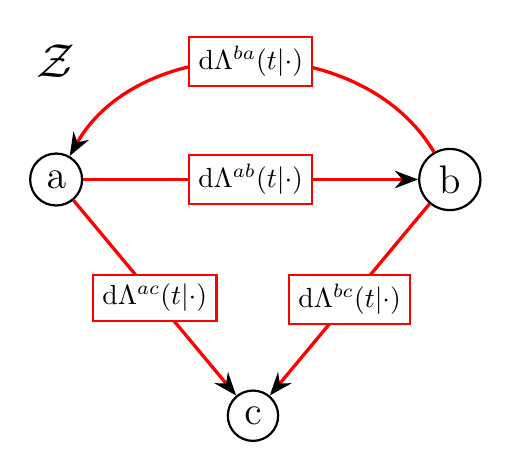
\begin{tikzpicture}
\begin{scope}[every node/.style={circle,thick,draw}]
    \node (A) at (0,0) {\Large a};
    \node (B) at (5,0) {\Large b};
    \node (C) at (2.5,-3) {\Large c};
\end{scope}
\begin{scope}
    \node (note) at (0,1.5) {\LARGE $\mathcal Z$};
\end{scope}
\begin{scope}[>={Stealth[black]},
              every node/.style={fill=white,thick,draw},
              every edge/.style={draw=red,very thick}]
    \path [->] (A) edge node {$\text d\Lambda^{ab}(t\vert \cdot)$} (B);
    \path [->] (B) edge node {$\text d\Lambda^{bc}(t\vert \cdot)$} (C);
    \path [->] (A) edge node {$\text d\Lambda^{ac}(t\vert \cdot)$} (C);
    \path [->] (B) edge[bend right=60] node {$\text d\Lambda^{ba}(t\vert \cdot)$} (A);
\end{scope}
\end{tikzpicture}
\caption{A representation of the chain discussed in sub-section \textit{\nameref{subsec:1}}}
\label{fig:1}
\end{wrapfigure}
We start by implementing the estimators for a simple model with three states say $\mathcal Z=\{a,b,c\}$ with $c$ being an absorbing state. We can thus identify the space $\mathcal J=\{1,2,3\}$ using the mapping $\psi$ given by $1\mapsto a$, $2\mapsto b$ and $3\mapsto c$ (see figure \ref{fig:1}). We assume that we have $L$ samples satisfying assumption 1:
\begin{align}
(\mathds 1_{\{Z_s^\ell=j\}},(Z_t^\ell)_{0\le t\le R},\tau^\ell \wedge R^\ell)_{\ell = 1,...,L}.
\end{align}
We also assume that $Z_0=a$ almost surely. We start by generating samples from a Markov chain that is time-inhomogeneous but on the form $\text d\Lambda(t)=\lambda(t)\mathbf M\ \text dt$. We know from lemma \ref{lem:prodsol}, that the product integral of such a Matrix and using the boundary condtion $\pi_0=(1,0,0)$ ($3\times 1$-matrix) we have that
\begin{align}
p(0,t)^\top=\pi_0^\top\exp\left(\mathbf M\int_0^t\lambda(u)\ \text du\right).
\end{align}
In the above $p(0,t)=(\mathbb P(Z_t=j))_{j\in\mathcal Z}$ and $\pi_0=p(0,0)$. In other words, we can easily compute the true values of the transition probabilities using regular matrix exponentiation. For this examples we choose
\begin{align}
    \lambda(t)=\frac{1}{1+\frac{1}{2}t} \quad\text{and}\quad \mathbf M=
    \begin{pmatrix}
        -3 & 2 & 1\\
        3 & - 4 & 1\\
        0 & 0 & 0
    \end{pmatrix}.
\end{align}
We start by sampling from this distribution using a censoring mechanism with $R\sim \text{Unif}(0,10)$ and an initial distribution $\pi_0=(1,0,0)$. We have layed out the code used in simulating the sample paths in appendix \ref{appendix:A1}.

\begin{table}[hbt!]\label{tbl:1}
\begin{center}
\begin{threeparttable}
\caption{The observations stored in \texttt{main\_df}}
\label{table_example}
\begin{tabular}{llllll}
\toprule
Id & Start\_Time & End\_Time & Start\_State & End\_State & Censored\\
\midrule
1 & 0 & 0.6 & 1 & 2 & FALSE\\
1 & 0.6 & 2 & 2 & 3 & FALSE\\
1 & 2 & $\infty$\tnote{a} & 3 & 3 & FALSE\\
\midrule
2 & 0 & 1 & 1 & 2 & FALSE\\
2 & 1 & 3 & 2 & 2 & TRUE\tnote{b}\\
2 & 3 & $\infty$ & 2 & 2 & TRUE\tnote{b}\\
\bottomrule
\end{tabular}
\begin{tablenotes}[hang] %use \tnote{a} for note a
%\item[]Table note
\item[a]The infinity sign indicates that the chain was absorbed at time 2.
\item[b]This indicates that the chain was censored at time 3 while $\psi(Z_{3-})=2$.
\end{tablenotes}
\end{threeparttable}
\end{center}
\end{table}

Recall, that the cumulative transition rates is the matrix exponent of the product of the integral of $\lambda$ over the interval and the matrix $\mathbf M$. We see that using a substitution argument with $y=1+\frac{1}{2}u$ hence $\frac{dy}{du}=\frac{1}{2}$ and thus
\begin{align}
\int_s^t\lambda(u)\ \text du=2\int_{1+\frac{1}{2}s}^{1+\frac{1}{2}t}\frac{1}{y}\ \text dy=2\log\left(1+\frac{1}{2}t\right)-2\log\left(1+\frac{1}{2}s\right).
\end{align}
Thus we can easily compare the Aalen-Johansen estimator with the true value of $p(0,t)$. In fact, we have that
\begin{align}
    p(0,t)^\top=(1,0,0)^\top \exp\left(2\log\left(1+\frac{1}{2}t\right)\mathbf M\right ).
\end{align}
Regarding estimation, we use a matrix-based approach and transform a main dataframe. Recall from theorem \ref{thm:2} that the Aalen-Johansen estimator is uniquely given by the product integral of the cumulative transition rates. And since the rates only changes on jump times of the observed chains, we get the result
\begin{align}
\text d_t\underbrace{\left( \prod_0^t\Big(\text{Id} +\text d_u \hat \Lambda^{(L)}(u\vert Z_s=j)\Big)\right)}_{:=\hat p^{(L)}(s,j,(0,t])}&=\hat p^{(L)}(s,j,(0,t])\Big(\text{Id} + \Delta\hat \Lambda^{(L)}(u\vert Z_s=j)\Big).
\end{align}
Thus on discontinuity points $\tau_i$ we have
\begin{align}
\hat p^{(L)}(s,j,(0,\tau_i])=\hat p^{(L)}(s,j,(0,\tau_i-])+\hat p^{(L)}(s,j,(0,\tau_i-])\Delta\hat \Lambda^{(L)}(\tau_i\vert Z_s=j).
\end{align}
Or entrywise we have the difference equation
\begin{align}
\hat p^{(L)}_{lk}(s,j,(0,\tau_i])&=\hat p^{(L)}_{lk}(s,j,(0,\tau_i-])+\sum_{m=1}^J \hat p^{(L)}_{lm}(s,j,(0,\tau_i-])\Delta \hat \Lambda^{(L)}_{mk}(\tau_i\vert Z_s=j)\\
&=\hat p^{(L)}_{lk}(s,j,(0,\tau_i-])+\sum_{m=1}^J \frac{\hat p^{(L)}_{lm}(s,j,(0,\tau_i-])}{\mathbb I_m^{(L)}(\tau_i-\vert Z_s=j)}\Delta\mathbb N^{(L)}_{mk}(\tau_i\vert Z_s=j).
\end{align}
We of cause have that
\begin{align}
\Delta\mathbb N^{(L)}_{mk}(\tau_i\vert Z_s=j)&=\frac{1}{Lg^{(L)}}\sum_{\ell = 1}^L\mathds 1_{\{Z_{\tau_i}^\ell = k\}}\mathds 1_{\{Z_{\tau_i-}^\ell = m\}}\mathds 1_{\{\tau_i<R^\ell \}},\\
\mathbb I_m^{(L)}(\tau_i-\vert Z_s=j)&=\frac{1}{Lg^{(L)}}\sum_{\ell = 1}^L\mathds 1_{\{Z_{\tau_i-}^\ell = m\}}\mathds 1_{\{\tau_i<R^\ell \}}.
\end{align}
Although we can ignore the fraction as they cancel out in $\Delta\mathbb N^{(L)}_{mk}(\tau_i\vert Z_s=j)/\mathbb I_m^{(L)}(\tau_i-\vert Z_s=j)$. Then we have
\begin{align}
\hat p^{(L)}_{lk}(s,j,(0,\tau_i])=\hat p^{(L)}_{lk}(s,j,(0,\tau_i-])+\sum_{m=1}^J \frac{\hat p^{(L)}_{lm}(s,j,(0,\tau_i-])}{\sum_{\ell = 1}^L\mathds 1_{\{Z_{\tau_i-}^\ell = m\}}\mathds 1_{\{\tau_i<R^\ell \}}}\sum_{\ell = 1}^L\mathds 1_{\{Z_{\tau_i}^\ell = k\}}\mathds 1_{\{Z_{\tau_i-}^\ell = m\}}\mathds 1_{\{\tau_i<R^\ell \}}
\end{align}
Thus by cleverly coding the function $\mathbb I^{(L)}_m(\tau_i- \vert Z_s=j)$ and $\Delta\mathbb N^{(L)}_{mk}(\tau_i\vert Z_s=j)$ we can easily implement the the function $\hat p^{(L)}_{lk}(s,j,(0,\tau_i])$ for all unique $\tau_i$.

Table \ref{tbl:1} show an example of an observation dataset of two observations. The first jumps from state 1 to state 2 at time 0.6 and then at time 2 to state 3, where i sojourns indefinetely. The other observation jumps to state 2 at time 1 and then is censored at time 3.

We start by calculating $\mathbb I^{(L)}_m(\tau_i- \vert Z_s=j)$ and $\mathbb N^{(L)}_{ml}(\tau_i- \vert Z_s=j)$ in the As-If-Markov case or $\mathbb I^{(L)}_m(\tau_i- )$ and $\mathbb N^{(L)}_{ml}(\tau_i-)$ in the Markov case. The code is given in appendix \ref{appendix:A2.2} and \ref{appendix:A2.3}. Then we may calculate the increments for the Nelson-Aalen estimator (see appendix \ref{appendix:A2.4}) and finally compute the transition probabilities $\hat p^{(L)}(s,j,(0,t])$ and $p(0,t]$ for the as-if case and Markov case respectively (see appendix \ref{appendix:A2.6}). For the estimates $\hat p^{(L)}(t\vert Z_s=j)$ we simply follow \ref{eq:5}.

\begin{figure}[h]
    \centering
    \includegraphics[width=0.95\textwidth]{Figures/plot1.png}
    \caption{The figure shows the conditional probabilities under a Markov assumption and As-If-Markov assumption. The dashed line is estimate from the As-If model, the  regular line is under the Markov assumption and the dots represent the true value. Based on $L=1,000$ samples. (code given in appendix \ref{appendix:A3})}
    \label{fig:2}
\end{figure}

As we can see in figure \ref{fig:2} both the Markov model and as-if Markov model does well in estimating the true transition probabilities $\mathbb P(Z_t=j\vert Z_s=i)$ (here tested for $Z_s=1$ for $s=0,1,3,6$). 

%\lipsum[1-4]
%\newpage

\printbibliography
\newpage

\appendix
\section{Source code}\vspace{-85pt}
\subsection{Simulating time-in-homogeneous Markov Chain}\label{appendix:A1}\vspace{-80pt}
\lstinputlisting[language=R,linewidth = 17cm, firstline=2, lastline=33]{Appendicies/A1.R}
\pagebreak

\subsection{Calculation of estimators}\label{appendix:A2}\vspace{15pt}
\subsubsection{Extraction of observations from \texttt{paths}, see \ref{appendix:A1}}\label{appendix:A2.1}\vspace{10pt}
\lstinputlisting[language=R,linewidth = 17cm, firstline=2, lastline=32]{Appendicies/A2.R}

\subsubsection{Calculation of $\mathbb I$}\label{appendix:A2.2}\vspace{10pt}
\lstinputlisting[language=R,linewidth = 17cm, firstline=33, lastline=64]{Appendicies/A2.R}

\subsubsection{Calculation of $\mathbb N$}\label{appendix:A2.3}\vspace{10pt}
\lstinputlisting[language=R,linewidth = 17cm, firstline=65, lastline=92]{Appendicies/A2.R}

\subsubsection{Calculation of Nelson-Aalen estimate}\label{appendix:A2.4}\vspace{10pt}
\lstinputlisting[language=R,linewidth = 17cm, firstline=93, lastline=111]{Appendicies/A2.R}

\subsubsection{Calculation of transition matrix $\prod_0^t\Big(\text{Id} + \text d_u \hat\Lambda(u)\Big)$}\label{appendix:A2.5}\vspace{10pt}
\lstinputlisting[language=R,linewidth = 17cm, firstline=112, lastline=128]{Appendicies/A2.R}

\subsubsection{Calculation of transition probabilities $\mathbf e_j\prod_s^t\Big(\text{Id} + \text d_u \hat\Lambda(u)\Big)$}\label{appendix:A2.6}\vspace{10pt}
\lstinputlisting[language=R,linewidth = 17cm, firstline=129, lastline=149]{Appendicies/A2.R}

\subsubsection{Calculation of conditional estimate}\label{appendix:A2.7}\vspace{10pt}
\lstinputlisting[language=R,linewidth = 17cm, firstline=150, lastline=208]{Appendicies/A2.R}

\subsubsection{Runtime}
\begin{table}[h]
    \centering
    \begin{tabular}{lccccc}
    \toprule
    Task & $n=1,000$ & $n=10,000$ & $n=100,000$ & $n=1,000,000$\\
    \midrule
    Simulation & 0.248 & 2.469 & 29.448 & 267.96\\
    \midrule
    \texttt{paths\_to\_df} & 0.066 & 0.465 & 2.249 & 33.675\\
    \texttt{df\_to\_I} & 0.059 & 0.176 & 2.437 & 42.078\\
    \texttt{df\_to\_N} & 0.029 & 0.049 & 0.702 & 5.884\\
    \texttt{N\_I\_to\_NA} & 0.002 & 0.011 & 0.489 & 2.082\\
    \texttt{NA\_to\_p} & 0.195 & 1.156 & 12.088 & 296.94\\
    \texttt{P\_conditioned} & 0.186 & 1.136 & 12.947 & 605.22 \\
    \midrule
    Total & 0.785 & 5.462 & 60.36 & 1550.779\\
    \bottomrule
    \end{tabular}
    \caption{In seconds. Run on R v. 4.3.0 on an Apple ARM64 M1 system with 8 GB ram.}
\end{table}
\pagebreak
\subsection{Plotting probabilities}\label{appendix:A3}\vspace{15pt}
\lstinputlisting[language=R,linewidth = 16cm, firstline=2, lastline=39]{Appendicies/A3.R}

\end{document}
